\documentclass[12pt]{article}
\usepackage[utf8]{inputenc}
\usepackage[T1]{fontenc}
\usepackage[a4paper,left=2cm,right=2cm,top=2cm,bottom=2cm]{geometry}
\usepackage[frenchb]{babel}
\usepackage{libertine}
\usepackage[pdftex]{graphicx}

\setlength{\parindent}{0cm}
\setlength{\parskip}{1ex plus 0.5ex minus 0.2ex}
\newcommand{\hsp}{\hspace{20pt}}
\newcommand{\HRule}{\rule{\linewidth}{0.5mm}}
\def\tab{$\>\>\>\>$}

\begin{document}

\begin{titlepage}
  \begin{sffamily}
  \begin{center}

    % Upper part of the page. The '~' is needed because \\
    % only works if a paragraph has started.
    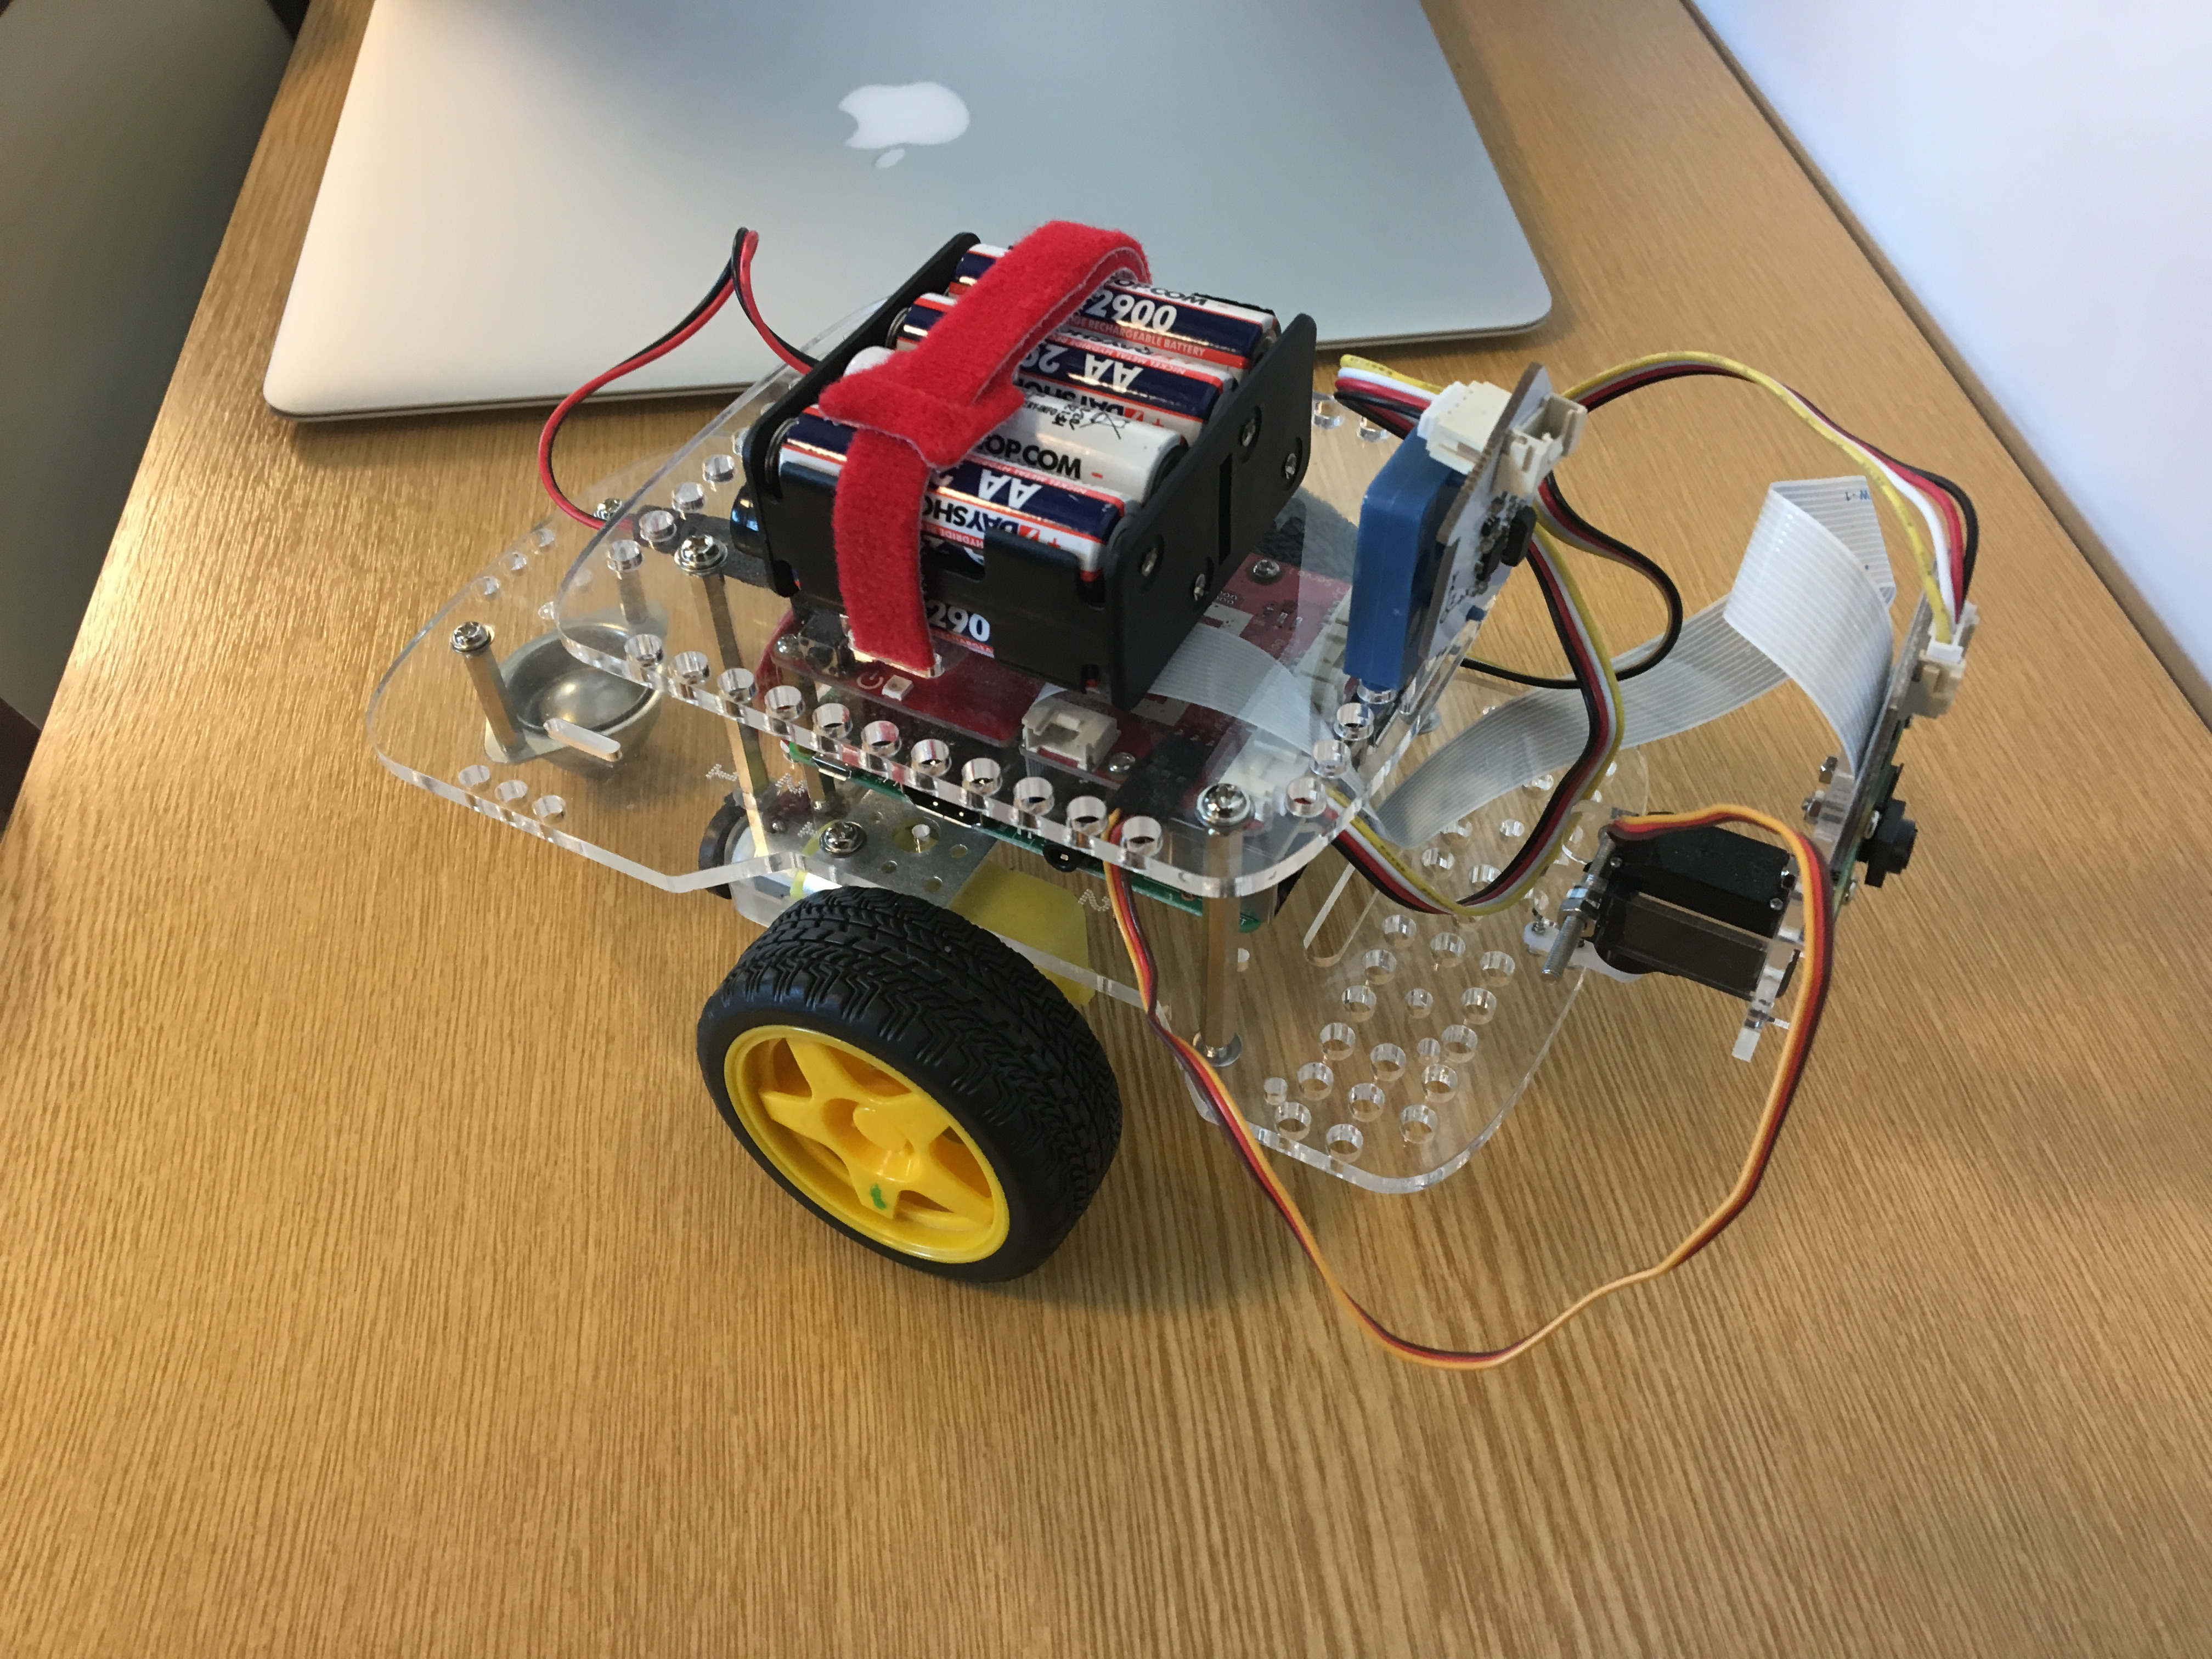
\includegraphics[scale=0.04]{IMG_8579.JPG}~\\[1cm] % mettre le logo de Sorbonne U à la place

    \textsc{\LARGE Sorbonne Université}\\[1cm]

    \textsc{\Large Licence d'informatique}\\[1.5cm]

    % Title
    \HRule \\[0.4cm]
    { \huge \bfseries Projet Robotique\\[0.4cm] }

    \HRule \\[1cm]
    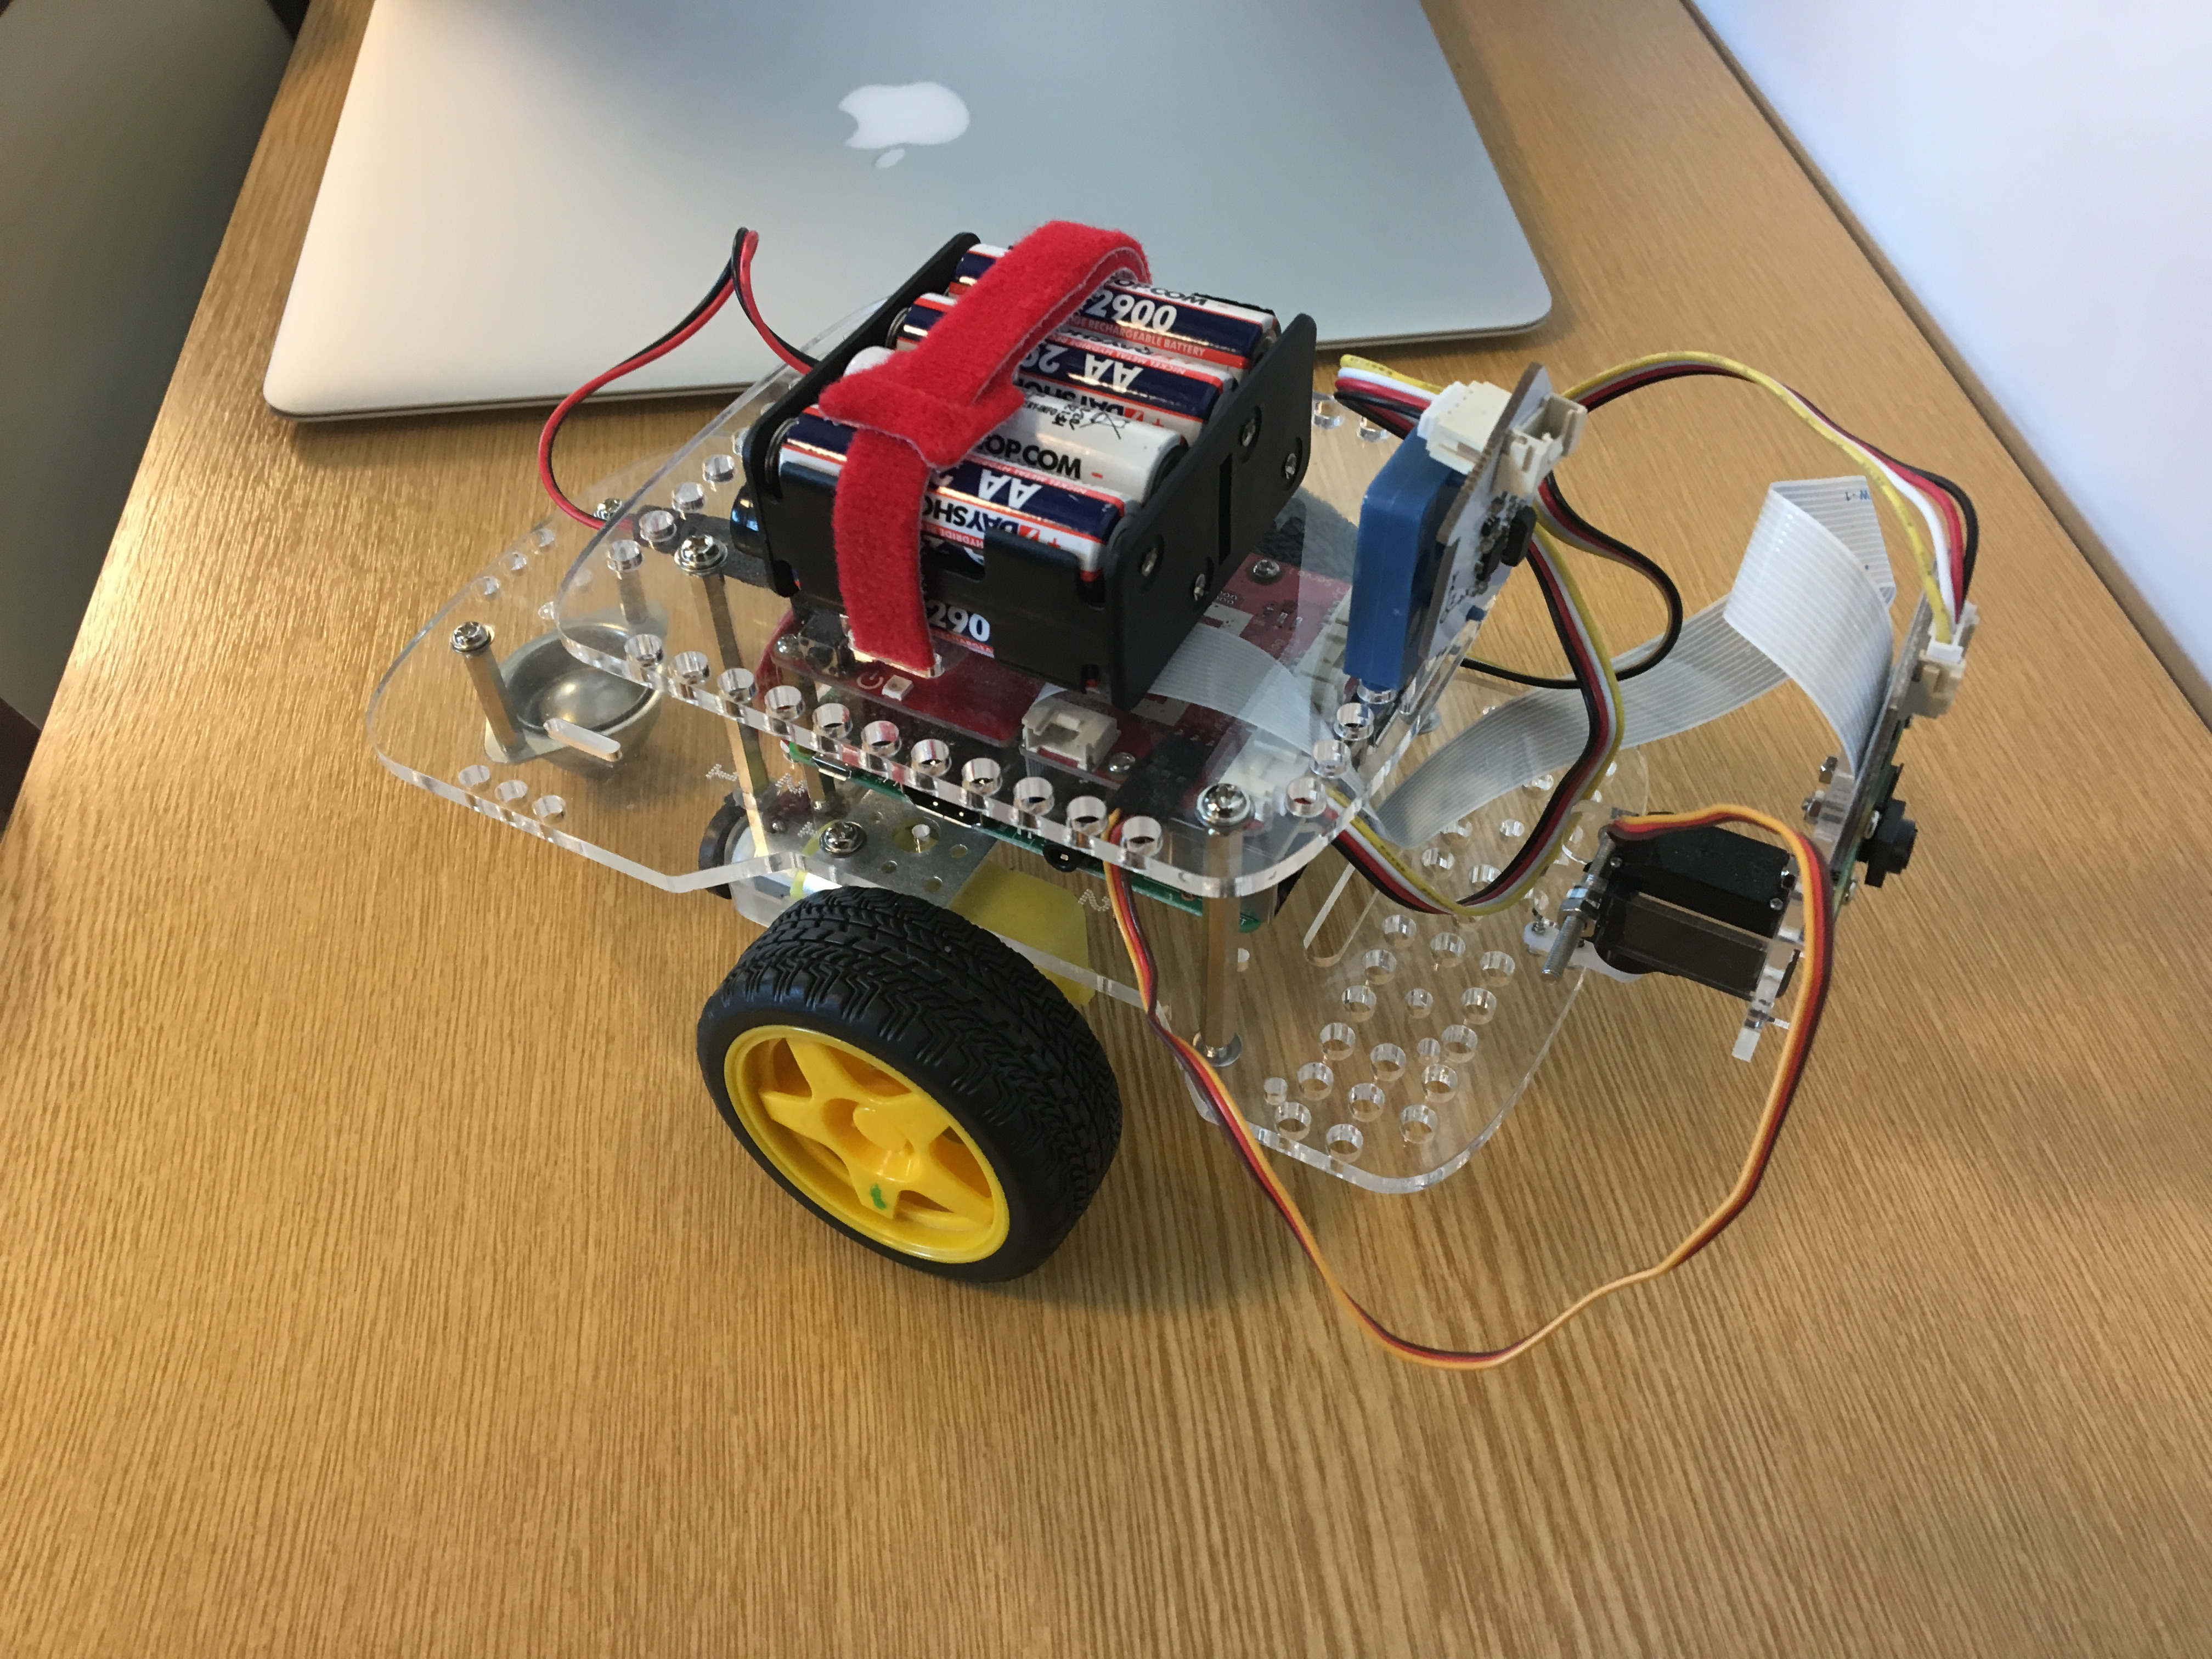
\includegraphics[scale=0.1]{IMG_8579.JPG}
    \\[0.5cm]

    % Author and supervisor
    \begin{minipage}{0.4\textwidth}
      \begin{flushleft} \large
        Groupe \textsc{FiveGuys}\\
        UE 2I013\\
      \end{flushleft}
    \end{minipage}
    \begin{minipage}{0.4\textwidth}
      \begin{flushright} \large
        \emph{Chargé de cours:} M. \textsc{Baskiotis}\\
        \emph{Chargé de TME:} M. \textsc{Veniat}
      \end{flushright}
    \end{minipage}

    \vfill

    % Bottom of the page
    {\large 1\ier{} Février 2019 — Mai 2019}

  \end{center}
  \end{sffamily}
\end{titlepage}

\tableofcontents
\newpage

\section{Introduction}

\tab Dans le cadre de l'UE 2I013, notre projet était de concevoir un logiciel permettant de contrôler un robot. Le projet était entièrement à notre charge aucun code ne nous était fourni. Le projet était construit de tel sorte que nos encadrants avait à la fois le rôle de nos superviseurs et de nos clients avec qui nous discutions des éléments a changer et de notre avancement dans le projet.

\tab L'objectif principal de ce projet était d'une part d'être un premier contact avec un projet de robotique et une découverte des méthodes de développement en équipe.

\tab Dans un premier temps, l'objectif est de mettre en place les briques de bases de notre projet comme le simulateur 2D et le moddèle physique ainsi que de mettre en place nos outils pour le bon déroulement du travail de groupe.

\tab Dans un second temps, une fois que notre modèle physique et notre simulateur étaient consédéré suffisament stable, nous avons commencé à développer les stratégies qui nous permettent de répondre aux challenges qui nous ont été soumis.

\newpage
\section{Rapport}
\subsection{Méthodes et outils}
\subsubsection{Agile/Scrum}
\tab Le cadre de notre projet n'était pas seulement le développement d'un logiciel de robotique, il avait également pour but de découvrir et mettre en place des méthodes efficaces pour le développement en équipe.

\tab En effet, dans les projets que nous réalisions jusqu'alors nous ne nous occcupions pas particulièrement de la façon dont nous allions gérer le développement de nos projets. Les codes à développer étaient relativement petit et guidé, en groupe de 2 à 3 personnes et sur quelques semaines seulement. Dans la plupart des cas nous avons donc réaliser nos projets d'un bout à l'autre pour obtenir directement notre rendu final avec une méthode dite "en V". Cette méthode consiste en un développement du projet de bout en bout afin à partir des exigence du "cahier des charges" (sujet) afin d'obtenir notre application. Le "retour client" se fait à la fin de celui-ci. Dans nos anciens projets celà ne possait pas problème mais dans le cadre de ce projet oui.

\tab Ce projet était construit de manière à ce que nous développions la totalité du code sur tout le semestre. Il nous fallait donc pouvoir avoir un retour régulier sur l'avancement afin de pouvoir modifier ce qui ne va pas dans la bonne direction et pouvoir s'adapter aux nouvelles exigences pour celui-ci. Nous avons donc chercher à appliquer une autre méthode qui nous a été présentée en cours, la méthode "Agile/Scrum".

\begin{center}



Schéma de la méthode Agile/Scrum.




\end{center}

\tab Nous avions donc pour objectif de mettre en place chaque semaine un ensemble de taches les plus petites et indépendantes possible les unes des autres nommées sprint. Les taches devaient toutes être définis avec un maximum de précisions et en concertation avec toute l'équipe pour qu'il n'y ai pas de différence de résultat en fonction du membre du groupe qui l'accompli. Elles ont toutes pour but de remplir un objectif de démonstration concrète de l'avancement du projet au client en terme de nouvelles fonctionnalités. L'objectif final de cette méthode était que chacun des membres du groupe puisse choisir les taches qu'il souhaite accomplir durant la semaine et qui seraient ensuite validées par un autre membre.

\tab A l'issue de la semaine, nous présentions une nouvelle démonstration au client pour obtenir ses retours. Grace aux retours client et au compte-rendu d'équipe rédiger dans la smeiane nous pouvions mettre en place le sprint de la semaine à venir.

\subsubsection{Outils pour le travail d'équipe}
\paragraph{Git \& GitHub\\}
\tab Pour pouvoir travailler de façon optimale et sécurisé ils nous fallait pouvoir développer sur un même code sans avoir à se le partager à chaque modifications. Nous avons donc utiliser le logiciel de gestion de version Git afin de conserver une version commune du code la plus à jour afin que chacun puisse travailler dessus à tout moment. La centrasation du code nous permet d'éviter un maximum de les conflits lors du développement du code et de conserver les versions précédentes du code au cas où nous aurions besoin de revenir sur une modification que nous avons apportées au projet et que posent problèmes.

\paragraph{Trello\\}
\tab Pour mettre en place les différentes taches du sprint de la semaine nous avons utiliser le logiciel Trello. Celui-ci nous a permi de rédiger nos cartes pour les différentes taches que nous avions dans notre sprint. Dans un prmier temps l'élaboration de nos sprints et la préparation de nos cartes n'étaient pas très au point ce qui nous conduisait à faire du travail en double où à une mauvaise compréhesion du résultat attendu.
\paragraph{Slack \& Whatsapp\\}
\subsubsection{Hiérarchie du code}

\begin{center}
Juste un schéma ?
\end{center}

\newpage
\subsection{Mise en place de briques de base}
\subsubsection{Modélisation du réel}
\subsubsection{Mise en place de l'interface graphique 2D}
\subsubsection{Stratégies de base}
\subsubsection{Passage de la simulation au réel}

\newpage
\subsection{Développement des stratégies}
\subsubsection{Stratégie carré}
\subsubsection{Stratégie détection de mur}
\subsubsection{Stratégie cercle}
\subsubsection{Stratégie contourner une porte}
\subsubsection{Stratégie détection balise}

\newpage

\section{Remerciements}

\newpage

\section{Conclusion}
\end{document}
